\chapter{Casi d'uso e workflow}

\section{Casi d'uso}

Nel seguente paragrafo verranno descritti i casi d'uso che l'applicazione supporta.

\subsection{Registrazione e login di un utente}

\textit{Deve essere possibile registrare un nuovo utente nel sistema e permettergli di autenticarsi.} \\

\noindent
Vi sono due tipologie di utenti, quelli interni all'ateneo (professori e studenti) e quelli esterni (aziende). Gli utenti interni devono effettuare l'accesso con il proprio account istituzionale utilizzando Google come provider federato, mentre le aziende possono inserire un'email qualunque. 

Una volta che un membro dell'ateneo esegue l'accesso mediante Google, viene reindirizzato indietro al sistema, che verifica l'email utilizzata nella fase di accesso a Google: se termina con \textit{@stud.unive} rappresenta un utente con il ruolo di studente, mentre se termina con\textit{@unive.it} rappresenta il un utente con il ruolo di professore. Una volta determinato il ruolo, il sistema verifica l'esistenza di un utente nella relativa \textit{collection} del database e in caso negativo lo crea, registrando un nuovo utente. A questo punto l'utente (professore o studente) è autenticato e viene indirizzato nella parte del portale protetta.

Per quanto riguarda un utente con il ruolo di azienda, invece, la procedura di \textit{login} e registrazione è divisa in pagine diverse. Nella pagina di registrazione l'utente deve indicare i dati della propria azienda, un'indirizzo email e una password, dopodiché verrà creato sia una nuova azienda che un nuovo utente, associando l'utente come amministratore della nuova azienda. Nella procedura di login invece, l'utente dovrà inserire l'email e la password utilizzate in fase di registrazione.

\begin{figure}[H]
	\centering
	\begin{subfigure}[b]{0.7\textwidth}
		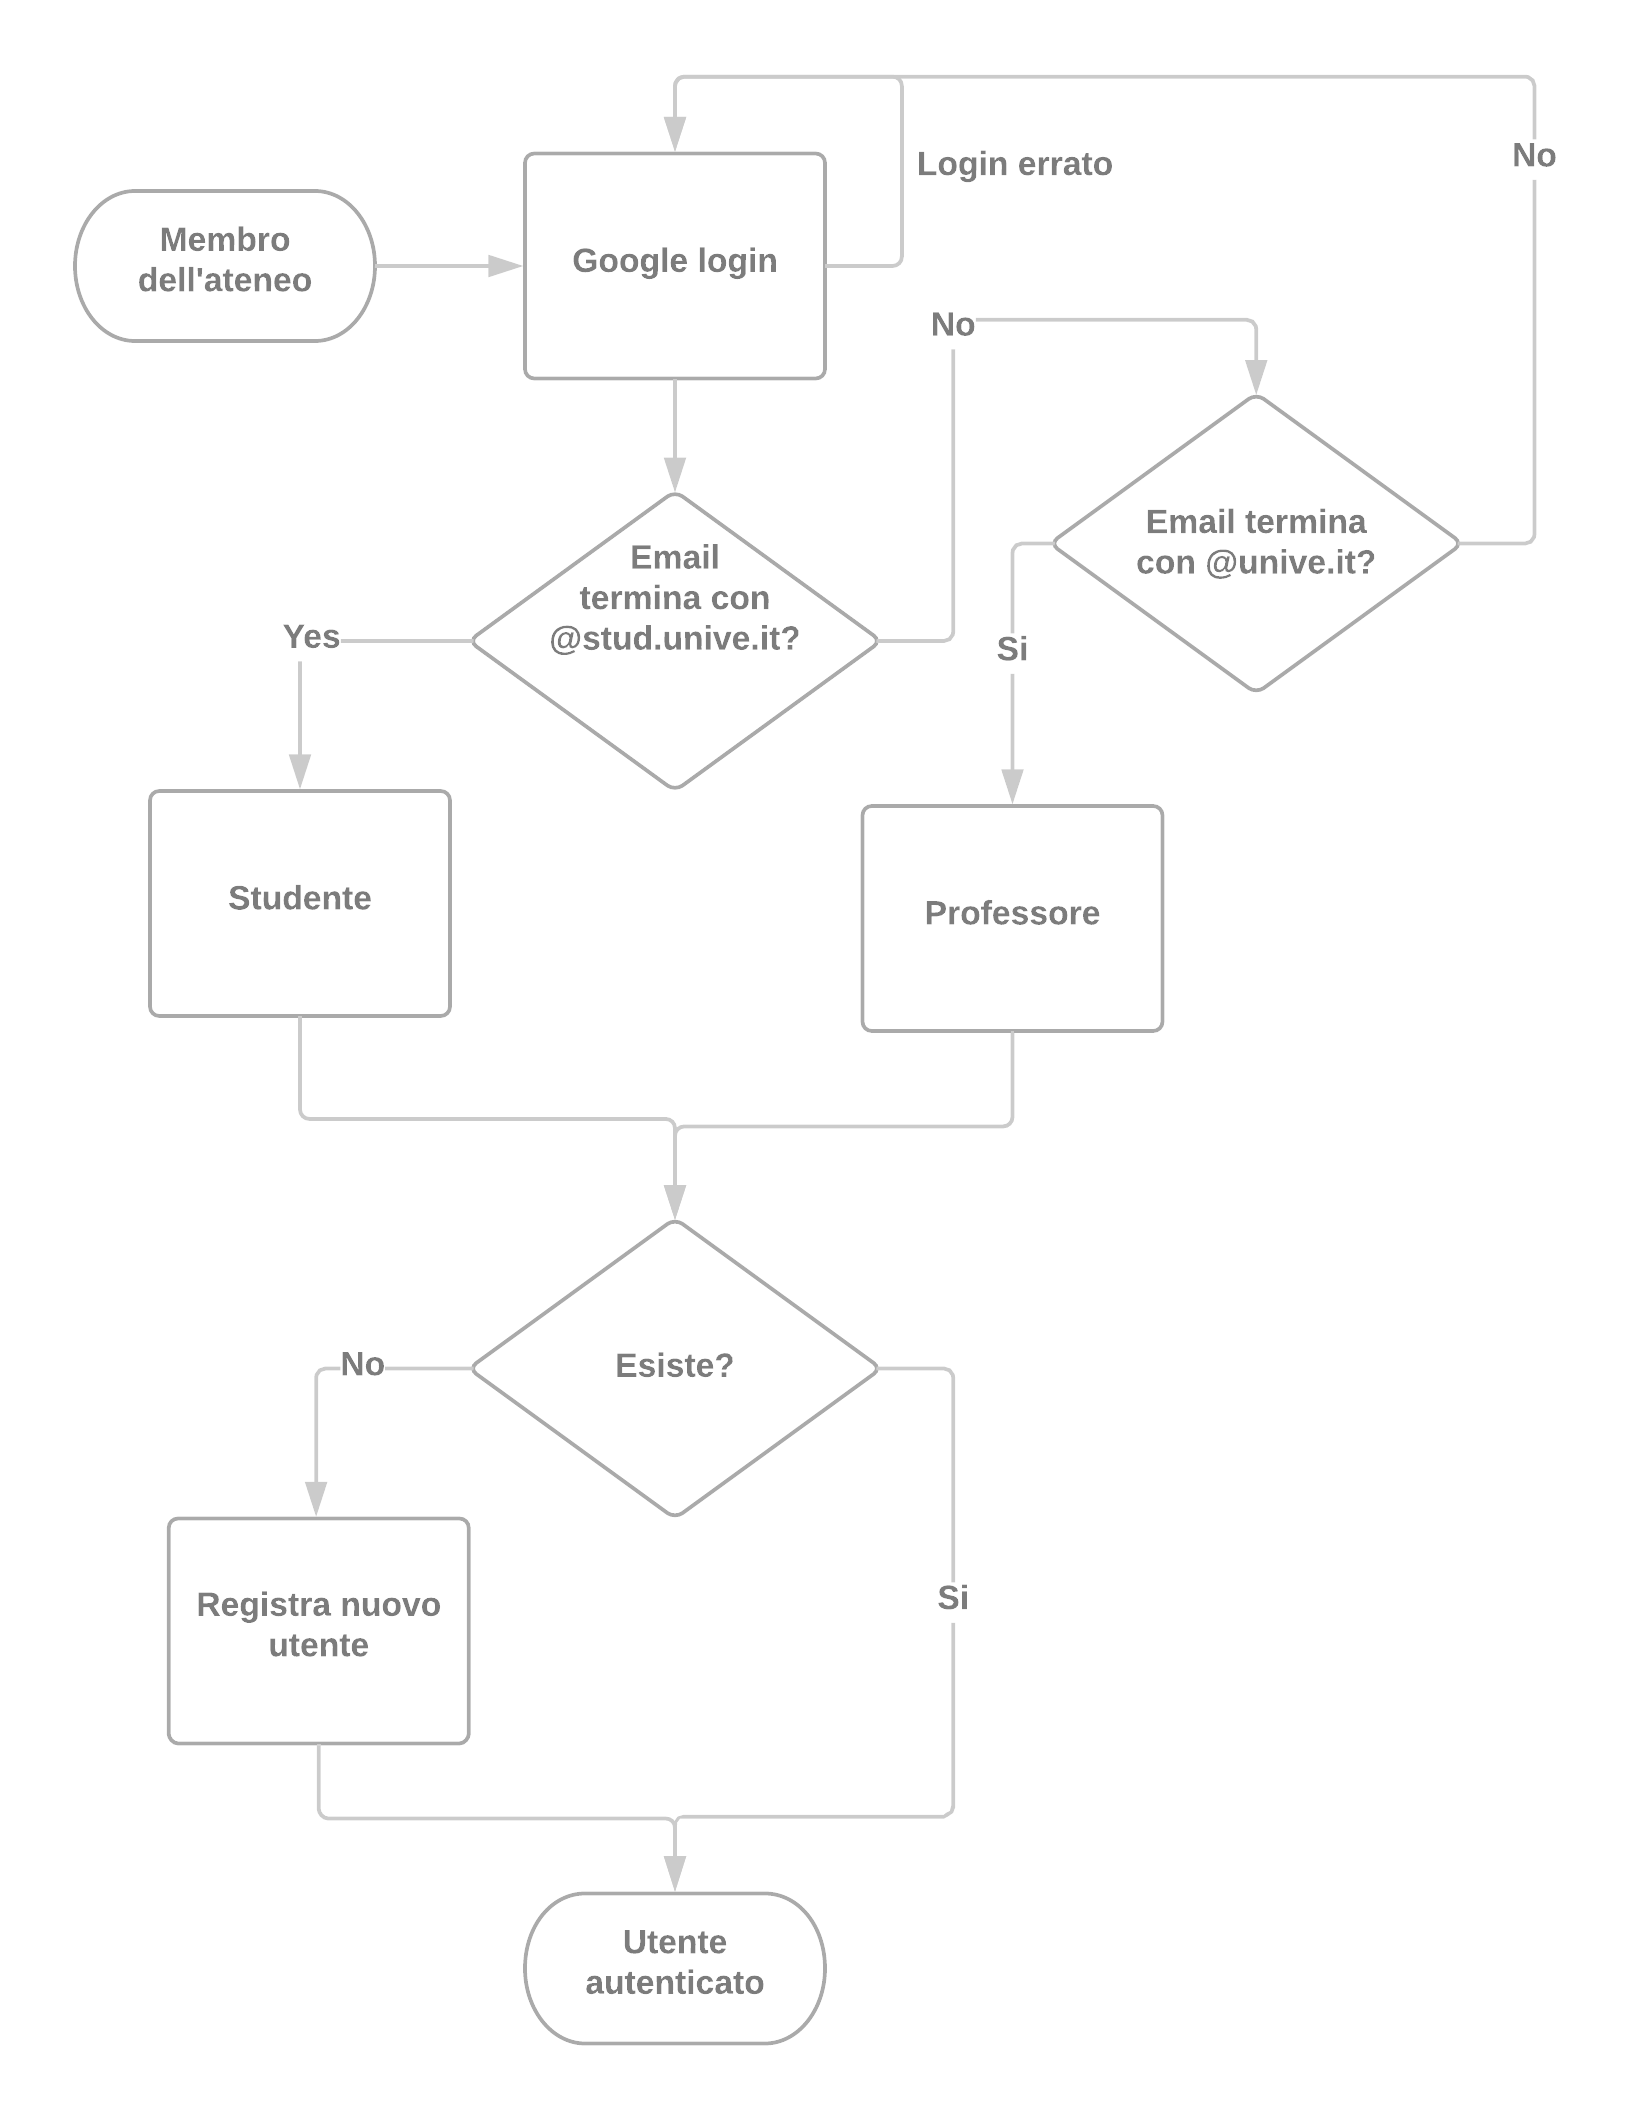
\includegraphics[width=\textwidth]{Chapter3/Figs/univelogin}
		\caption{Membro dell'ateneo}
		\label{fig:univelogin}   
	\end{subfigure}             
	\begin{subfigure}[b]{0.7\textwidth}
		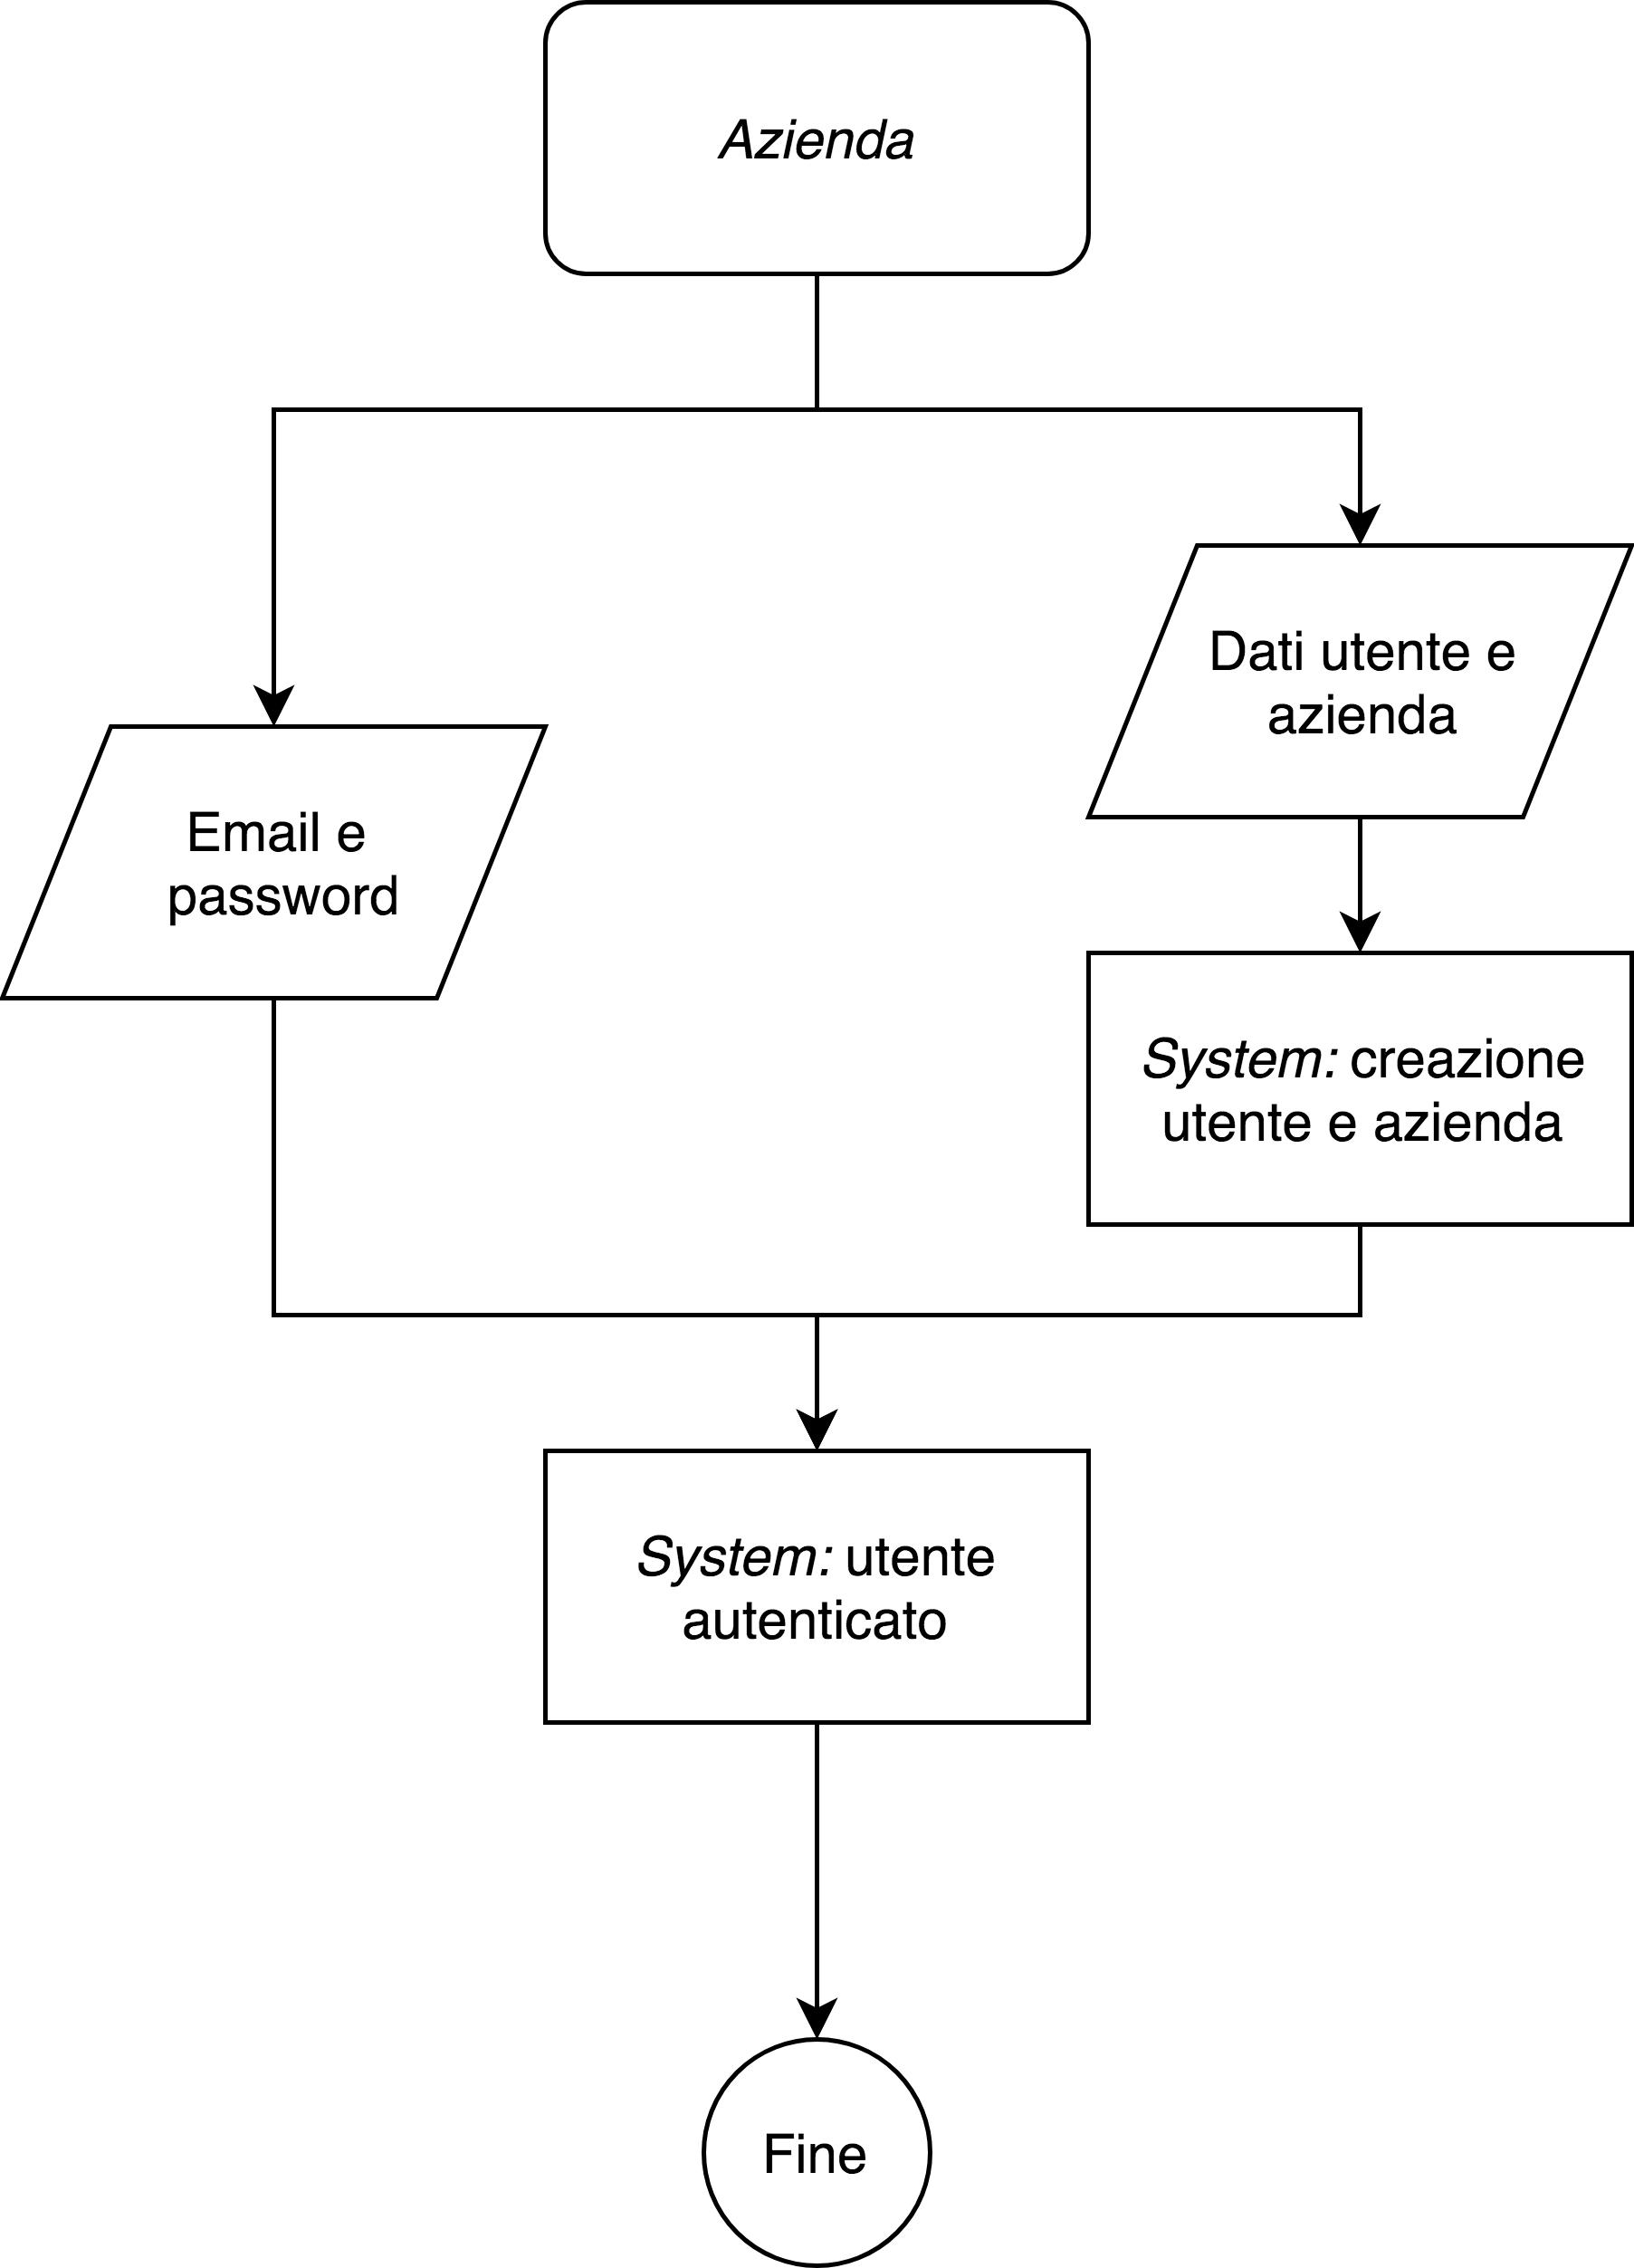
\includegraphics[width=\textwidth]{Chapter3/Figs/companylogin}
		\caption{Azienda}
		\label{fig:companylogin}
	\end{subfigure}
	\caption[Flusso di login e registrazione di un utente]{Flusso di login e registrazione di un utente}
	\label{fig:uc-login}
\end{figure}

\subsection{Creazione  e modifica di un tirocinio}


\textit{Deve essere possibile --- per un utente con il ruolo azienda --- l'aggiunta una nuova offerta di tirocinio.} \\

\noindent
Una volta effettuato l'accesso con le proprie credenziali, sarà sufficiente navigare all'indirizzo \textit{"/auth/internship/add"} seguendo la voce di menù "Tirocini > Aggiungi tirocinio". Apparirà una pagina con un \textit{form} che permette l'inserimento di un'offerta. Una volta salvata, prima di essere pubblicata deve essere approvata da un professore. Prima di essere approvata o rifiutata, vi sono le possibilità di modifica e cancellazione dell'offerta, raggiungibili seguendo le voci di menù "Azienda > I miei tirocini".

\subsection{Approvazione di un tirocinio}

\textit{Deve essere possibile --- prima che venga pubblicata --- approvare o rifiutare un'offerta di tirocinio di un azienda da parte di un professore.} \\

\noindent
Una volta che un'azienda pubblica una nuova offerta, essa è visibile da tutti gli utenti con il rolo di professore alla pagina \textit{"/auth/internship/approve"}, raggiungibile dalla voce "Professore > In attesa di approvazione". Da questa pagina, che contiene una tabella, è possibile approvare o rifiutare singolarmente le offerte visionandone il contenuto.

\subsection{Candidatura ad un tirocinio}

\textit{Deve essere possibile per uno studente candidarsi ad un'offerta di tirocinio pubblicata da un azienda.} \\

\noindent
Una volta effettuato l'accesso, lo studente può visualizzare tutte le offerte di tirocinio pubblicate. Una volta selezionata quella di suo gradimento, può (se vi sono ancora posti liberi) candidarsi indicando un professore suo referente. La candidatura di effettua tramite il pulsante "Candidati" a fondo pagina di un'offerta di tirocinio. Una volta avviata la candidatura, il professore indicato dovrà accettarla o rifiutarla e solo successivamente sarà rimbalzata all'azienda per la conferma finale.

\subsection{Approvazione candidatura (professore)}

\textit{Deve essere possibile per un professore visualizzare, accettare e rifiutare le proposte di candidatura che lo coinvolgono come referente.} \\

\noindent
Una volta effettuato l'accesso, il professore può recarsi alla pagina \textit{"/auth/proposals/professor"} dalla voce "Professore > Studenti in attesa" e visualizzare tutte le candidature che lo coinvolgono. Può accettarle o rifiutare singolarmente accedendo alla pagina di dettaglio.

\subsection{Approvazione candidatura (azienda)}

\textit{Deve essere possibile per un'azienda visualizzare, accettare e rifiutare le proposte di candidatura alle proprie offerte di tirocinio.} \\

\noindent
Una volta effettuato l'accesso, l'azienda può recarsi alla pagina \textit{"/auth/proposals/company} dalla voce "Azienda > Proposte ricevute" e visualizzare tutte le candidature che lo coinvolgono. Può accettarle o rifiutare singolarmente accedendo alla pagina di dettaglio.

\subsection{Avvio di un tirocinio}

\textit{Deve essere possibile, una volta che sia il professore che l'azienda hanno approvato una candidatura di uno studente, Avviare il tirocinio per iniziare a tracciarlo.} \\

\noindent
Una volta individuato il tirocinio in questione, sarà sufficiente entrare nella pagina di dettaglio della candidatura e premere il pulsante "Avvia tirocinio". Da questo momento in poi sarà possibile completare il foglio presenze e terminare il tirocinio.

\subsection{Compilazione foglio presenze}

\textit{Deve essere possibile, una volta avviato un tirocinio, completare il foglio delle presenze dello studente.} \\

\noindent
Una volta individuato il tirocinio in questione, sarà sufficiente entrare nella pagina di dettaglio della candidatura, spostarsi all'interno della sezione "Foglio presenze" e premere il pulsante "Aggiungi". Verranno chiesti data e ore lavorare e un nuovo record sarà aggiunto alla tabella.

\subsection{Terminazione di un tirocinio}

\textit{Deve essere possibile, una volta avviato un tirocinio, terminarlo.} \\

\noindent
Una volta individuato il tirocinio in questione, sarà sufficiente entrare nella pagina di dettaglio della candidatura e premere il pulsante "Termina candidatura". Da questo momento sarà possibile generare le documentazione associata al tirocinio eseguito.

\subsection{Generazione documentazione}
\textit{Deve essere possibile, una volta terminato un tirocinio, generarne la relativa documentazione precompilata in PDF..} \\

\noindent
Una volta individuato il tirocinio in questione, sarà sufficiente entrare nella pagina di dettaglio della candidatura e premere il pulsante "Genera documentazione". Verrà aperta una nuova finestra del browser contenente il documento PDF precompilato contenente i dettagli del tirocinio, dell'azienda, del professore, dello studente e la tabella del foglio presenze.


\section{Ciclo di vita di un tirocinio}
\begin{figure}[H]
	\centering
	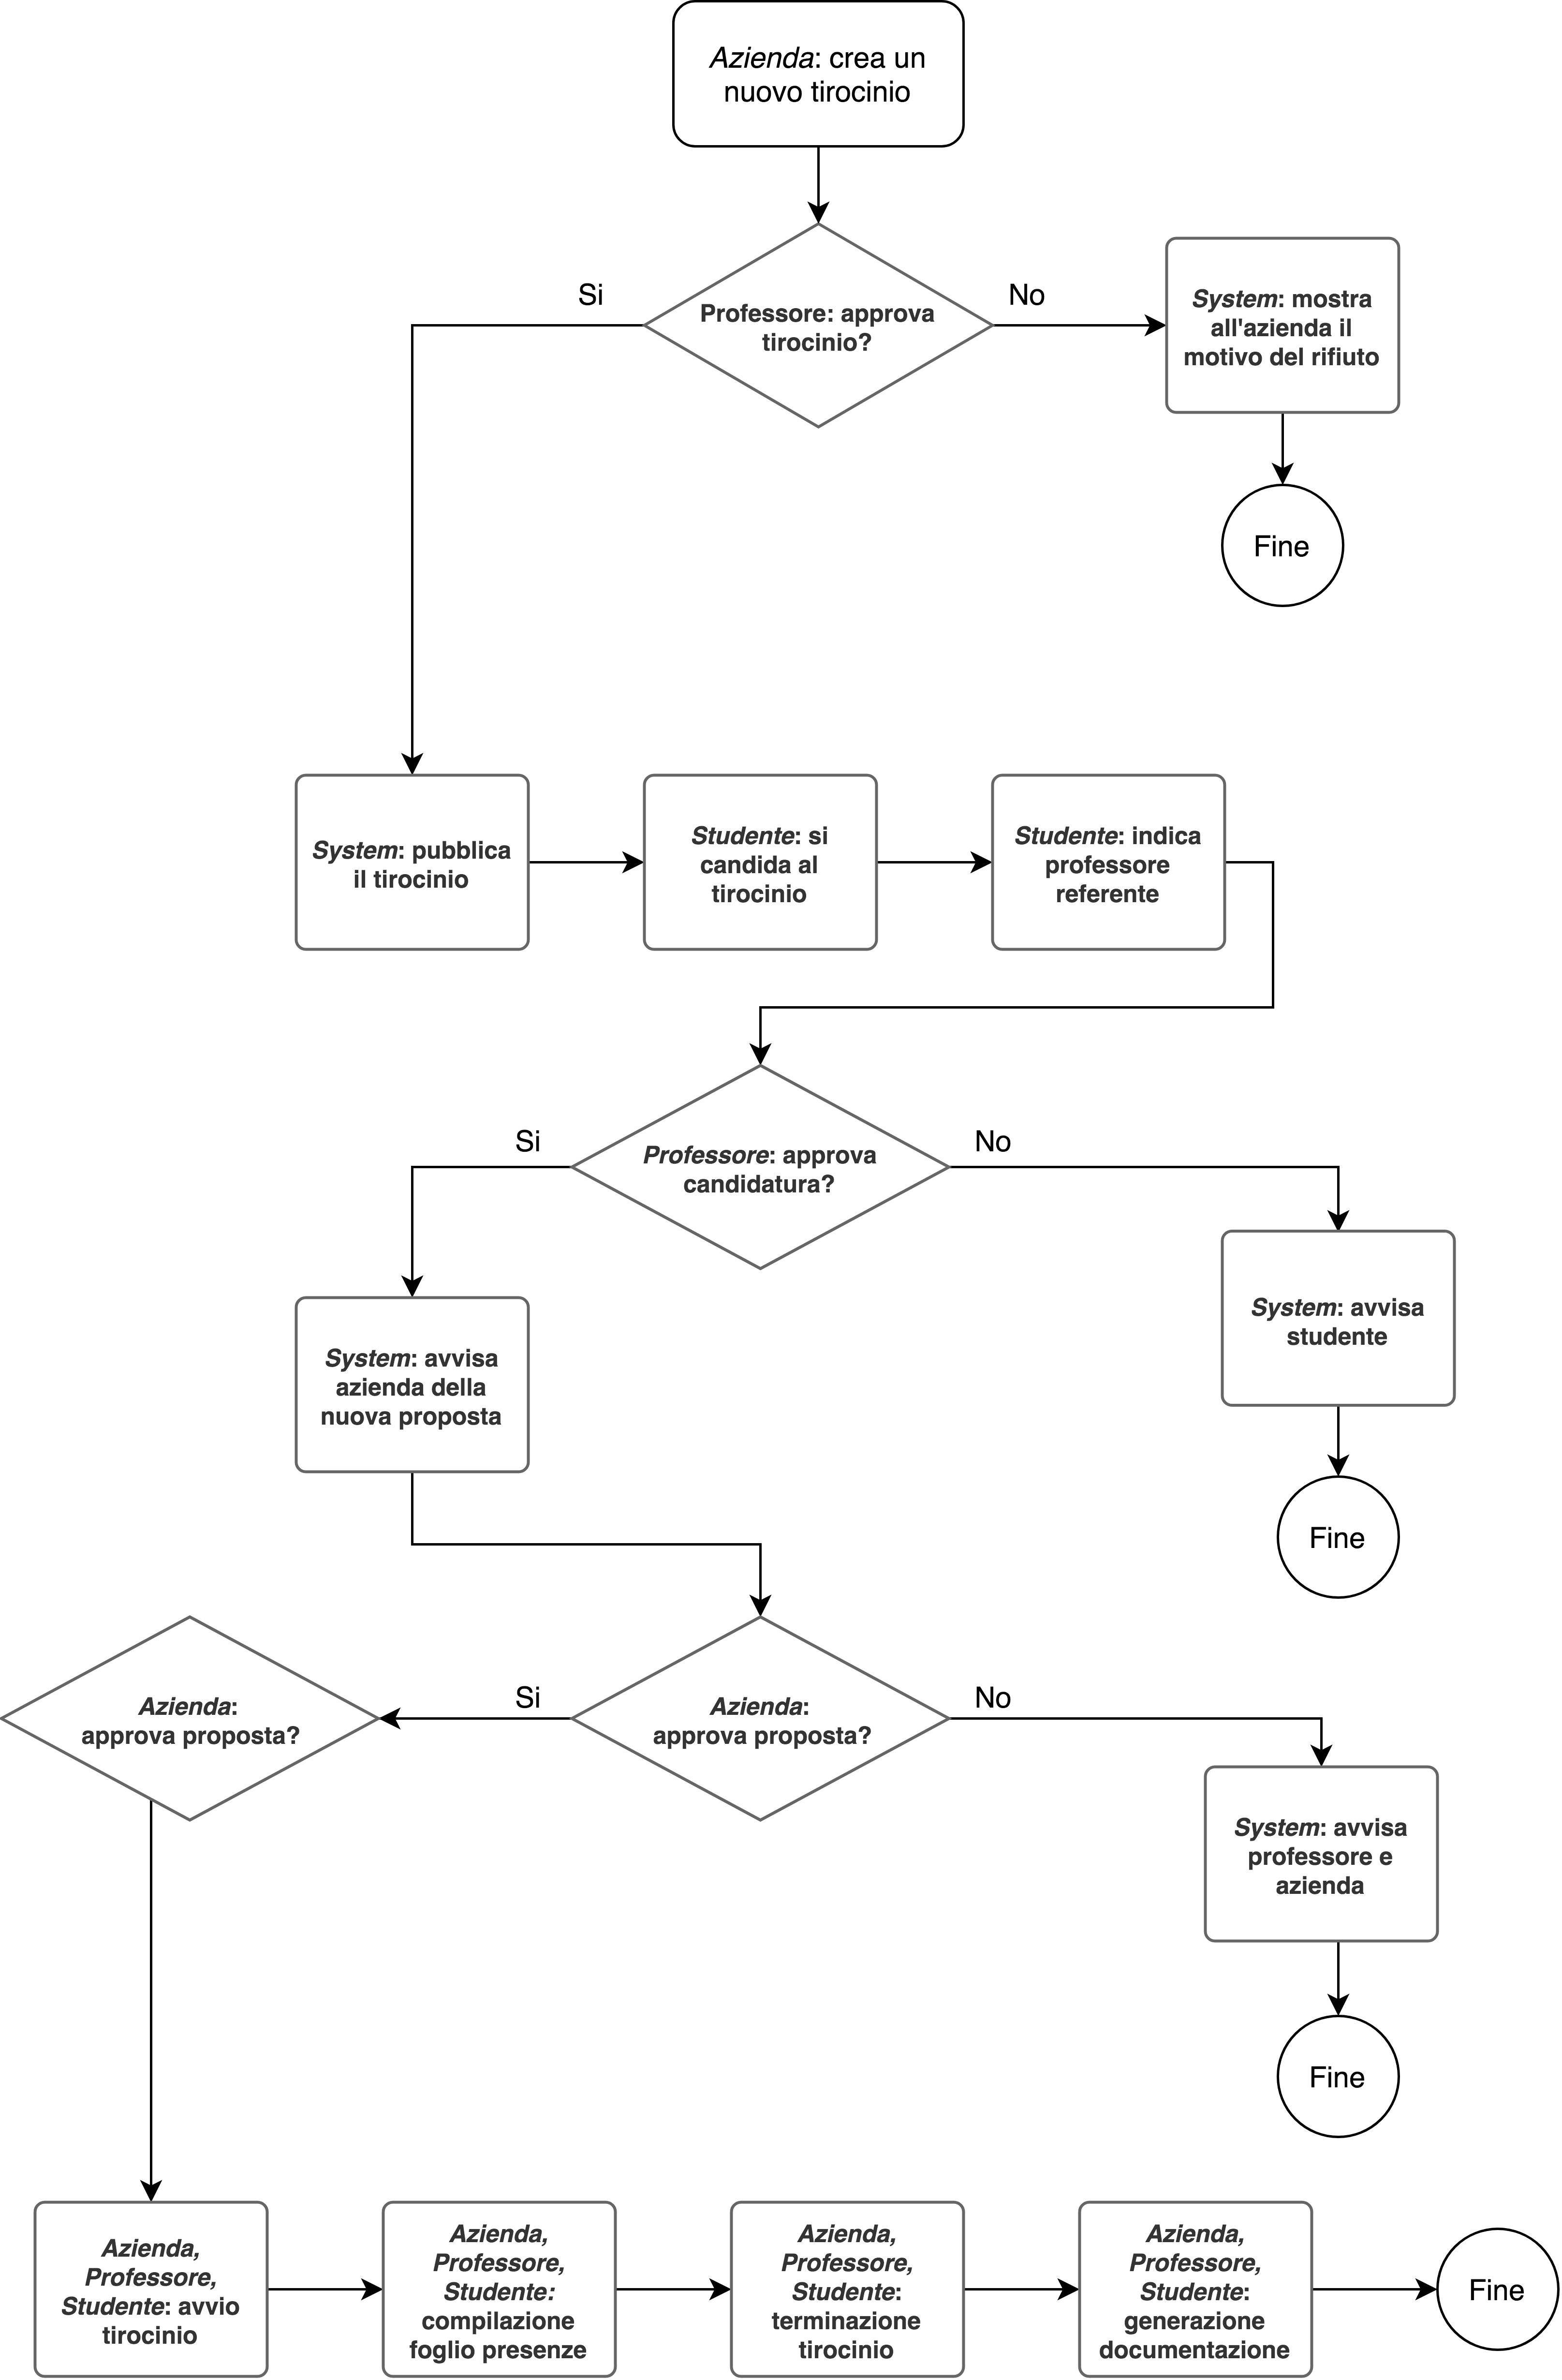
\includegraphics[width=0.8\textwidth]{Chapter3/Figs/states-flaw}
	\caption[Ciclo di vita di un tirocinio]{Ciclo di vita di un tirocinio}
	\label{fig:workflaw}
\end{figure}